\chapter{Analyse \& Design ( 25 \%)}
\label{chap:design}

Im vorhergehenden Kapitel wurden Ziele und Leistungskriterium für das CI-System festgelegt.
Diese sollen nun auf konzeptueller Ebene umgesetzt werden.
Dazu wird zuerst ein Überblick des Gesamtkonzeptes gegeben.
Anschließend werden Besondere Konzepte zur 
%XXX: continue


\section{Grundlegende Systemarchitektur}
\label{sec:design:sysarch}
Diese Sektion gibt Aufschluss über die Grobstruktur des CI-Systems auf logischer und physischer Ebene.

\subsection{logisch}

\begin{figure}[ht]
  \centering
  \label{fig:grob-layout-komponenten-logisch}
  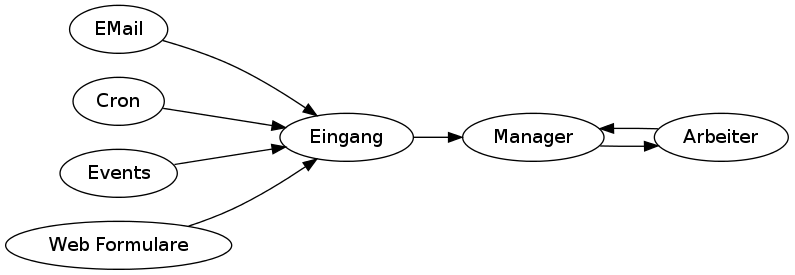
\includegraphics[width=\textwidth]{imageinput/grob-layout-komponenten-logisch.png}
  \caption{\"Ubersicht ber Systemkomponenten - logisch}
\end{figure}


Die erste wichtige Komponente ist der Eingang,
in ihm gehen Aufträge aus verschiedensten Quellen ein.
Nach dem sie validiert wurden, werden die Aufträge an
die zweite wichtige Komponente, den Manager, weitergegeben.
Dort werden sie vorbereitet und entsprechend der Build-Matrix Arbeitspakete erstellt.
Nun treten Manager und Arbeiter in eine Interaktion,
um zu bestimmen welcher Arbeiter das Eigentliche Arbeitspaket bearbeitet.
Anschließend werden die Arbeitspakete von den jeweilig designierten Arbeitern abgefertigt.

%XXX: more


\subsection{physisch}

\begin{figure}[ht] 
  \centering
  \label{fig:grob-layout-komponenten}
  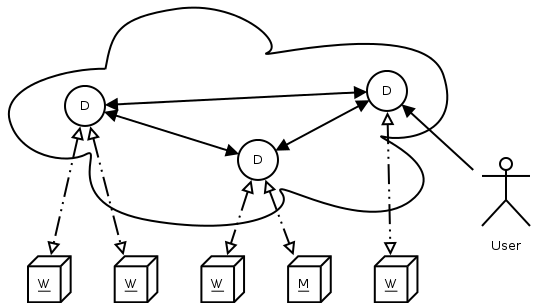
\includegraphics[width=\textwidth]{imageinput/grob-layout-komponenten.png}
  \caption{Übersicht über Systemkomponenten - physisch}
\end{figure}

Der physische Aufbau unterscheidet sich stark von den bisher dagewesenen CI-Systemen.
Grund ist der Fokus auf die verteilte Datenbank, direkte Kommunikation
wird der Interaktion mit einer verteilten Datenbank weichen.

Das System besteht somit aus Komponenten welche alle als Clients einer verteilten Datenbank operieren.
Die Abbildung~\ref{fig:grob-layout-komponenten} zweigt die Struktur.
Nennenswert ist dabei die Bindung einer Komponente and bestimmte Datenbank-knoten,
dies dient der Kontrolle der Lokalität und wird später noch vorgestellte Verfahrensweisen unterstützen.

%XXX more

\section{Grundlegendes Datenschema}


\begin{figure}[ht] 
  \centering
  \label{fig:datenstrukturen}
  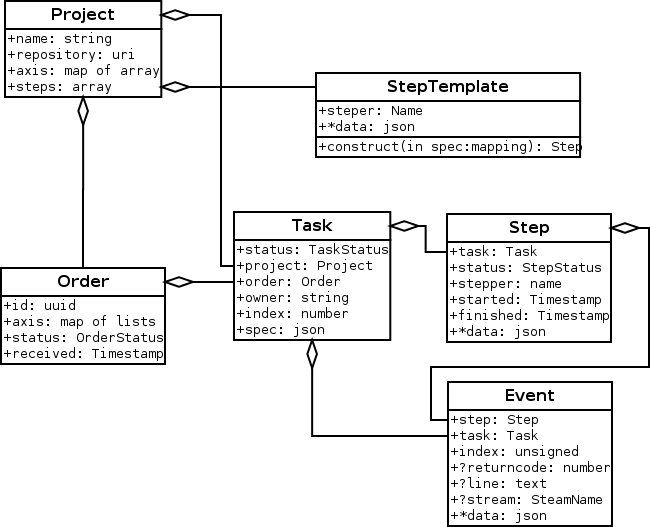
\includegraphics[width=\textwidth]{imageinput/datenstrukturen-step-templates.png}
  \caption{Grundlegende Datenstrukturen}
\end{figure}

Das grundlegende Datenschema, in Abbildung~\ref{fig:datenstrukturen} als UML Klassendiagramm dargestellt,
beschreibt die Daten des Kernsystems und einige ihrer Interaktionen.

Die wichtigsten Datentypen sind dabei Projekt, Auftrag (Order),
Arbeitspaket (Task) und Arbeitsschritt (Step).

\subsubsection{Projekt}

Das Projekt beinhaltet neben dem Namen auch alle Informationen,
die später für das Erstellen von Arbeitspaketen sowie
die Ausführung einer Integration benötigt werden.
Dazu gehört das Quellcode-repository (repo), von dem später
die Quelltexte für das dem Test unterworfenen Projekt bezogen werden.
Weiterhin beinhaltet es die Build-Achsen,
welche die Wertebereiche der einzelnen Ebenen der Build-Matrix
beschreiben.

\subsubsection{Arbeitsschritt Templates}

Der mitunter wichtigste Teil eines Projektes ist jedoch die Beschreibung der Arbeitsschritte als Templates.
Die Darstellung als Template ist dabei bewusst gewählt,
sie ermöglicht es jedem Arbeitspaket speziell konfigurierte Arbeitsschritte zur Verfügung zu stellen.
Außerdem bewirkt die erneute Speicherung in der Datenbank,
das Bearbeiten der Schritte eines Projektes keinen Einfluss auf bereits erstellte Arbeitspakete hat.
Zudem stellen die extra Objekte auch einen Anschlusspunk für die Datensammlung dar.
Die Methode \textit{construct} des Templates dient dazu,
einen Arbeitsschritt, angereichert mit einer entsprechenden Konfiguration, zurückzugeben.

\subsubsection{Auftrag}

Ein Auftrag beinhaltet grundsätzlich eine Referenz auf das zugehörige Projekt,
außerdem beinhaltet er Überschreibungen/Zusätze für die Build-Achsen,
dies Ermöglicht es sowohl in den Achsen eingeschränkte,
als auch erweiterte Aufträge zu erstellen.
Diese werden später genauer erklärt.
Zusätzlich beinhaltet der Auftrag einen Status, dieser beinhaltet den aktuellen Stand der Bearbeitung.

\subsubsection{Arbeitspaket}
%XXX: eventuell projekt hier nicht referenzieren
Ein Arbeitspaket beinhaltet neben Referenzen zu dem Projekt und dem Auftrag,
seine Spezifikation. Diese gibt die Ausbildung aller Build-Achsen für dieses Paket an.
des weiteren beinhaltet es den Index, dieser gibt die Numerische Position in der Build-Matrix an.
Auch ein Arbeitspaket hat einen Status, welcher den aktuellen Bearbeitung-stand zum Ausdruck bringt.
Zudem bestimmt das Feld ``Owner'' den Arbeiter, welcher das Arbeitspaket letztendlich bearbeiten wird.

\subsubsection{Arbeitsschritt}

Ein Arbeitsschritt referenziert das zugehörige Arbeitspaket.
Neben den Zeitpunkten für Anfang und Ende seiner Ausführung,
benennt er im Feld ``stepper'' um welche Art von Arbeitsschritt es sich handelt.
Das Feld ``status'' gibt Auskunft über den aktuellen Stand der Bearbeitung.
Das Feld ``data'' soll weitere dynamische Informationen zum Ausdruck bringen,
die bei der Ausführung genutzt werden.

%XXX: dies dient \ldots


\subsubsection{Event}
%XXX referenz auf task?

Das Event bringt Datensammlung zur Laufzeit zum Ausdruck.
Neben den Referenzen für den Arbeitsschritt und das Arbeitspaket,
beinhaltet es eine Indexnummer und einen Timestamp.
Die Indexnummer ist eine aufsteigende Zahl
und gibt den Events eines bestimmten Arbeitsschritts eine feste eindeutige Reihenfolge.
Der Timestamp gibt den Events eine zeitliche Ordnung (welche jedoch nicht eindeutig ist).


Zusätzlich zu diesen Basisdaten, beinhaltet ein Event beliebige weitere optionale Felder.
Einige mögliche (und ihre Datentypen) sind:

\begin{description}
    \dhitem[returncode: Number] Rückgabe-wert eines Prozesses bei seiner Beendigung.
    \dhitem[line: Text] Textzeile eines Datenstromes der Ausgabe
    \dhitem[lineno: Number] Zugeh. Zeilennummer
    \dhitem[stream: Name] Zugeh. Name des Datenstromes
    \dhitem[start: Name] Mitteilung über den Start eines best. Vorganges
    \dhitem[end: Name] Mitteilung über den Abschluss eines best. Vorganges
\end{description}




\section{Grundlegende Logik der Komponenten}

Diese Sektion behandelt die grundlegende Logik  der Einzelteile des Systems,
sie bilden die Bausteine für das Gesamtsystem.

%XXX MORE

\subsection{Auftragsannahme}

Der Auftragsannahme lässt sich grob in 2 Abschnitte einteilen.
Zuerst geht ein Auftrag ein, was je nach Methode in mehrere Schritte beinhalten kann,
danach wird er überprüft und damit angenommen oder abgelehnt.


\begin{figure}[ht]
  \centering
  \label{fig:lebenszyklus-auftrag-eingang}
  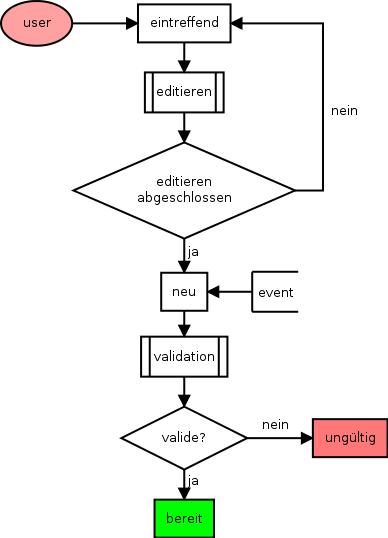
\includegraphics[height=5in]{imageinput/lebenszyklus-auftrag-eingang.png}
  \caption{Auftragsannahme: Flussdiagramm}
\end{figure}


\subsubsection{Eingang}

Auftragseingang gestaltet sich in der Praxis vielseitig.
Da nicht alle Quellen direkt einen fertigen Auftrag generieren können,
beginnt ein Auftrag im Zustand eingehend, sind schließlich alle Daten zusammengekommen,
so wird der Eingang festgehalten und der Auftrag wird vom System weiterverarbeitet.

%XXX Quellen betrachten``


\begin{verbatim}
- quellen
- editiern
- typisches
-> eine auswaehlen
\end{verbatim}

\subsubsection{Validation}

%XXX: genauer beschreiben

Die Validation verfolgt das Ziel, Aufträge auch aus weniger vertrauenswürdigen Quellen anzunehmen.
Dies ermöglicht Verwendung ähnlich zu TravisCI, was es erlaubt, Zuarbeiten von Außenstehender zu Testen.
Für die Überprüfung stehen verschiedene Möglichkeiten zur Verfügung.
Ein Eingang per Mail/Mailingliste oder Pull-Request auf einer Code-Hosting,
kann z.b. nach erstmaliger Erlaubnis, wiederholt zugelassen werden,
während Informationen die Mitarbeiter einsenden z.b. an ihr Arbeitsverhältnis gebunden werden können.

Zeitgesteuerte Eingänge innerhalb des Systems können jedoch grundsätzlich zugelassen werden.

Den Abschluss der Validation stellt die Markierung des Auftrages als Valide oder invalide dar.

\subsection{Management}

\begin{figure}[ht] 
  \centering
  \label{fig:lebenszyklus-auftrag-abarbeitung}
  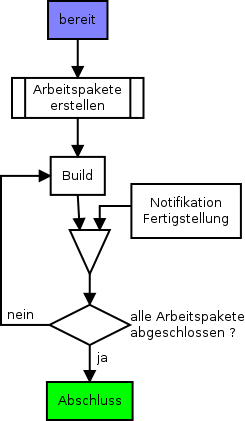
\includegraphics[height=4in]{imageinput/lebenszyklus-auftrag-abarbeitung.png}
  \caption{Auftragsannahme: Flussdiagramm}
\end{figure}

\subsubsection{Auftragsvorbereitung}

In der Auftragsvorbereitung werden Details aus dem Projekt zum Auftrag hinzugefügt.
Die vordefinierten Build-Achsen werden vom Projekt übertragen.
Dies stell sicher, dass der Aufrag und sein Umfang eindeutig bestimmt sind,
bevor mit der Erstellung von Arbeitspaketen begonnen wird.


\subsubsection{Bereitstellung von Arbeitspaketen}

Das Bereitstellen von Arbeitspaketen stellt den Anfang der eigentliche Arbeitsphase dar.
Entsprechend der Werte der Build-Achsen des Auftrages, werden nun die Arbeitspakete generiert,
wobei jedes Arbeitspaket eine der Wertekombinationen darstellt.
Nachdem alle Arbeitspakete erstellt sind, ist die Bearbeitung des Auftrages an sich abgeschlossen.

\subsubsection{Abschluss von Aufträgen}

Der Abschluss eines Auftrages ist ein Ereignis, welches Impliziert werden kann.
In im zu entwickelnden System wird der Abschluss eines Auftrages definiert,
als der Zustand der Eintritt, wenn alle Arbeitspakete eines Auftrages
einen finalen Zustand erreichen.

Dies Vereinfacht die Behandlung des Auftragsabschlusses,
da man nicht nach Abschluss von Arbeitspaketen weitere Operationen durchführen muss,
um den eventuellen Abschluss festzustellen.

\subsection{Zuteilung/Abarbeitung von Arbeitspaketen}


\subsubsection{Lebenszyklus eines Arbeitspaketes}


\begin{figure}[ht] 
  \centering
  \label{fig:lebenszyklus-arbeitspaket}
  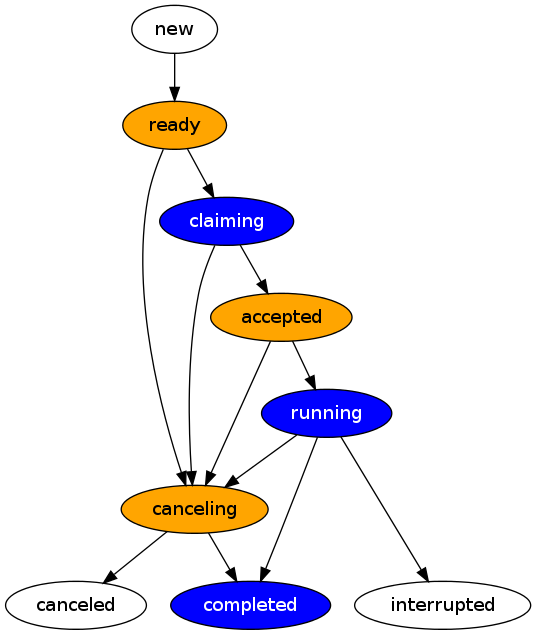
\includegraphics[height=4.5in]{imageinput/lebenszyklus-arbeitspaket.png}
  \caption{Lebenszyklus eines Arbeitspaketes bei Ausschreibungen}
\end{figure}


\subsubsection{Vorbereitung Abarbeitung}

\subsection{Überblick Methoden der Zuteilung}


\begin{verbatim}
- diese sektion besch. sich mit


- methoden
    - token basiert
    - ausschreibungsbasiert

\end{verbatim}


\subsubsection{Melde verfahren}

\begin{verbatim}
- arbeiter teilen nur mit, dass sie arbeitsfaehig sind
- manager kontrolliert wer welchen auftrag erhaelt
cons:
    - fuer erweiterte use-cases extra wissen im manager notwendig
\end{verbatim}

\begin{figure}[ht] 
  \label{fig:auftrag-zuteilung-token}
  \begin{sequencediagram}
      \newinst{worker}{:Worker}
      \newinst[1]{manager}{:Manager}
      \mess{worker}{token <spec>}{manager}
      \mess{manager}{work <spec>}{worker}
      \mess{worker}{result}{manager}
  \end{sequencediagram}
  \caption{Auftragszuteilung: Tokenbasiert}
\end{figure}

\subsubsection{Ausschreibungsverfahren}

\begin{verbatim}
- manager teilt offene auftraegeposten mit (in datenbank verf.)
- arbeiter konkurieren um offene auftraege
- manager entscheidet wer den aufrag dann erhaelt


- autonomere arbeiter
- manager muss nur noch entscheiden wer, nicht mehr warum
- aufgrund der datenbank konzeptuell einfacher -> beweis oder weg
\end{verbatim}

\begin{figure}[ht] 
  \label{fig:auftrag-zuteilung-claim}
  \begin{sequencediagram}
      \newinst{workera}{:Worker A}
      \newinst[1]{manager}{:Manager}
      \newinst[1]{workerb}{:Worker B}
      \mess[1]{manager}{availiable}{workera}
      \prelevel
      \prelevel
      \mess[1]{manager}{availiable}{workerb}

      \mess[1]{workera}{claim}{manager}
      \prelevel
      \prelevel
      \mess[2]{workerb}{claim}{manager}
      %XXX: better call?
      %\prelevel
      %\prelevel
      %\begin{call}{manager}{approve}{manager}{workera}
      %\end{call}
      \mess{manager}{approve A}{workera}
      \prelevel
      \mess{manager}{approve A}{workerb}
  \end{sequencediagram}
  \caption{Auftragszuteilung: Ausschreibungsbasiert}
\end{figure}


\subsubsection{Abschluss Abarbeitung}

- ende der arbeisschritte
- zusammenfassung resultat
- endscheidung fehlschlag oder nucht


\subsection{Abarbeitung von Arbeitspaketen}

\begin{verbatim}
- lineare abarbeitung
- abbrich bei fehlschlag
\end{verbatim}

\subsubsection{Arbeitsschritte}


\begin{figure}[ht] 
  \centering
  \label{fig:lebenszyklus-arbeitsschritt}
  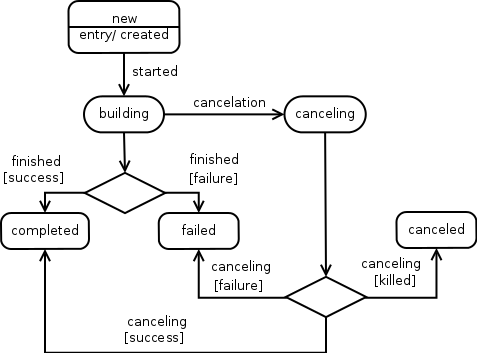
\includegraphics[height=3.4in]{imageinput/lebenszyklus-arbeitsschritt.png}
  \caption{Stategraph eines Arbeitschrittes}
\end{figure}

\begin{verbatim}
- kill wird in der impl nicht betrachtet

\end{verbatim}


\subsubsection{Datensammlung zur Laufzeit}

\begin{verbatim}
- sinn/echtzeit?

- beispielhaft
    - STDOUT/ERR
    - exakte testresultate/reports
\end{verbatim}

\subsubsection{Datensammlung nach Abschluss eines Schrittes}

Datensammlung nach dem Abschluss eines Arbeitsschritts,
Umfasst in der Regel verschiedenste Dateiformate.
Diese werden aus den verschiedensten Gründen generiert.
Üblich sind Test-Resultate, Logdateien, Build-Resultate und Archive.

Die Abbildung dieser Datensammlung kann dabei auf 2 Arten geschehen,

\begin{enumerate}
    \item als Teil des Schrittes
    \item als eigene Art von Schritt
\end{enumerate}

Die Abbildung als eigene Art von Arbeitsschritt,
hat einige Vorteile, da sie die Zuständigkeit vom reinen Arbeitsschritt
und dem Daten-sammeln sauber trennt.

Dies macht die Werkzeuge zur Datensammlung wesentlich einfacher.
Anstatt sie in jeden Schritt integrieren zu müssen,
kann einfach nach dem Schritt angewendet werden.


\subsubsection{Abschluss von Arbeitsschritten}



- returncodes
- fehler

\section{Besondere Ansätze zur Datenbank-Interaktion}

%XXX: http://dbmsmusings.blogspot.de/2010/04/problems-with-cap-and-yahoos-little.html


\subsection{CAP Abdeckung}

Wie bereits in Sektion~\ref{sec:base:cap} erwähnt,
ist es immer nur möglich 2 der 3 Aspekte des CAP Theorems abzudecken.

Jedoch ist es durchaus legitim für verschiedene Teile
einer verteilten Applikation unterschiedliche Bereiche abzudecken.
Sobald genau definiert ist, für welche Daten in welchem Kontext welche Eigenschaften benötigt werden,
kann ein konsistentes Modell geschaffen werden.

Wichtig ist bei dieser Betrachtung, dass die unterschiedlichen Komponenten des Entwickelten CI-Systems
nicht zwingend eine direkte Konsistenz-Bindung untereinander benötigen.
Wichtig ist nur, die Konsistenz zwischen einer Komponente
und dem Datenbank-knoten, mit dem sie Kommuniziert.

Das Haupt-system, in dem alle Komponenten in Kommunikation stehen,
%XXX: s1?
soll nach Systemanforderung \textbf{S1} immer verfügbar sein und somit einen Teil-Ausfall  verkraften.
Somit kommt für die Kommunikation zwischen Komponenten nur das Modell \textbf{A-P} in Frage
(was Verfügbar und Partitionstolerant bedeutet).

Die Anbindung einzelner Komponenten and ihre Datenbank-knoten, hat jedoch andere Anforderungen.
Da eine direkte Anbindung and die Datenbank für das Funktionieren einer Komponente unabdingbar ist,
kann in diesem Fall nur das Modell \textbf{C-A} zum Einsatz kommen.


%XXX: http://www.infoq.com/articles/cap-twelve-years-later-how-the-rules-have-changed


\subsection{Status-Maschinen zur Wahrung der Konsistenz}

%XXX: Literatur
% http://blog.incubaid.com/2012/10/25/caulking-your-distributed-algorithm-implementation/
\nocite{statechart}

Statusmaschienen sind ein allgemein bekanntes Werkzeug,
um den den Ablauf eines komplexen Programms zu beschreiben oder zu erklären.
In der Regel wird dazu ein sog. StatusGraph verwendet.
Dieser ist ein Gerichteter Graph der die Zustände und Zustandsänderungen eines Systems beschreibt.

Wie bereits in Abbildung \ref{fig:lebenszyklus-arbeitspaket} gezeigt,
stellt der Lebenszyklus eines Arbeitspaketes einen solchen Statusgraph dar.
Als Besonderheit ist er sogar frei von Zyklen.
Dadurch ist es unmöglich den gleichen Status noch einmal zu erreichen.

Bindet man Zusätzlich noch die Transitionen an bearbeitende Knoten (Agenten außerhalb der Datenbank),
so ist es auch bei einer Partitionierung der Datenbank eine Konsistenz der Gesamtsystems gewährleistet.

%XXX: moar?


Mit dem dem Eingang und der Abarbeitung von Aufträgen verhält es sich ähnlich,
jedoch ist der Graph dort Wesentlich einfacher.
Die Abbildungen \ref{fig:lebenszyklus-auftrag-eingang} und \ref{fig:lebenszyklus-auftrag-abarbeitung} zeigen den groben Ablauf.
Der Wechselpunkt zwischen Eingang und Abarbeitung ist die der Validation angeschlossene Markierung zur Bereitschaft.
Da es nur diesen einen Punkt des Austausches gibt, ist die Wahrung der Konsistenz des Auftrages denkbar einfach,
Mit der Bereitschaft, wird die Verantwortung vom Eingang zur Abarbeitung übertragen.

\subsection{Abbildung des Verteilten Systems auf Datenbanken}




\subsection{Auftragsverteilung}

\section{Logisches Gesamtkonzept}
\subsection{Eingang}
\subsection{Management}
\subsection{Arbeiter}

\section{Arbeitsschritte und der Kontext ihrer Ausführung}

\subsection{Überblick und grundlegender Ablauf}

\begin{figure}[h!]
  \centering
  \label{fig:klassen-arten-arbeitsschritt}
  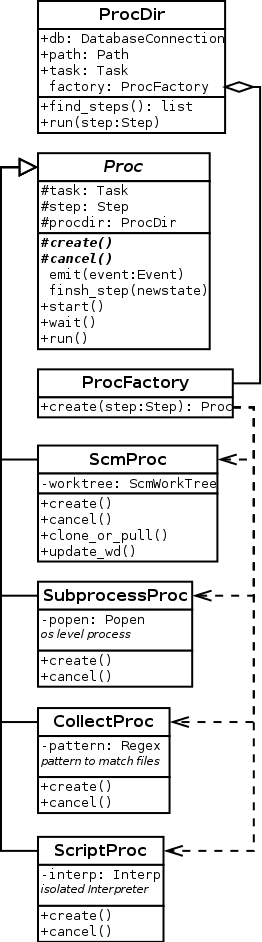
\includegraphics[height=\textheight]{imageinput/klassen-arten-arbeitsschritt.png}
  \caption{Arten und Ablauf von Arbeitsschritten}
\end{figure}

Wie man auf der Grafik~\ref{fig:klassen-arten-arbeitsschritt} gut erkennen kann,
bildet das Arbeitsverzeichniss (ProcDir) die Basis
für die Durchführung der Arbeitsschritte eines Auftrages.

Es bindet alle Operationen, die notwendig sind,
um die Kontrolldaten (Steps, siehe Fig~\ref{fig:datenstrukturen})
aus der Datenbank zu laden und diese dann an Ausführende Objekte zu binden (Proc).

Der Lebenszyklus eines Proc Objektes wird dabei

%XXX: More

\subsection{Prozess Schritte}

Die Aufgabe eines Prozessschrittes ist es,
einen Programm mit vorgegebenen Parametern auszuführen.
Dies ist auch der Grund, warum der ``ProcessProc'' Datentyp einen
Prozess-Handle enthält.

Dabei Fallen zur Laufzeit sammelbare Daten wie z.B. Text auf den Standard Eingabe-/Ausgabe Datenströmen an.
Außerdem verändern sich statistische Informationen über den Prozess wie Speicher-verbrauch, IO-Last, u.a.


\subsection{Skript Schritte}

Skript-Schritte unterscheiden sich von Prozess-Schritten in der Hinsicht,
dass sie kein Programm an sich, sondern ein Skript ausführen.
Daher können sie in die Lage versetzt werden,
weitere Laufzeit-Daten zur Verfügung zu stellen


\subsection{Quellcode Management Schritte}

Interaktion mit dem Quellcode-Management behandelt die grundlegenden Operationen mit denen. %XXX MORE
Es wird, wenn notwendig ein Arbeitsverzeichniss erstellt.
Danach gibt es mehrere Grundlegende Operationen, die durchgeführt werden können.

\begin{description}
    \dhitem[Eingang von Historie]
        bringt die lokale Historie auf den aktuellen Stand, ``pull'' genannt

    \dhitem[Aktualisierung des Arbeitsverzeichniss]
        aktualisiert die Dateien im Arbeitsverzeichniss
        auf eine gewünschte Version
    \dhitem[Anwendung von Patches]
        wendet Patches auf das aktuelle Arbeitsverzeichniss an
\end{description}

\subsection{Datensammlungs Schritte}

Datensammlung-schritte haben die Aufgabe,
bei vorhergehenden Schritten entstandene Dateien 
in die Datenbank zu überführen.
Die Grundfunktion pflegt dabei nur den Inhalt der Datei ein.
Laufzeit-Daten dieses Schritts sind die gefundenen Dateien.

Dabei wird das Pattern verwendet, um festzustellen, ob eine Datei, %XXX more

Erweiterte Versionen dieser Schritt-Art, könnten zusätzliche Funktionen,
wie z.b. Einpflegen von Testergebnissen aus JunitXML Dateien in die Datenbank,
übernehmen

\section{Erweiterungen}
\subsection{Analyse Test-Resultate}
\subsection{Analyse Verhalten eines Programms}


\section{Benutzeroberfläche}

% kann krit
% kein tolles
% nur werkzeuge


\section{Zusammenfassung}

was kommt
was kommt nicht
